\documentclass{aa}
\usepackage[varg]{txfonts}
\usepackage[separate-uncertainty=true]{siunitx}
\usepackage[version=3]{mhchem}

\sisetup{
    range-units         = brackets,
}


\def\eps{\varepsilon}
\def\aap{A\&A}
\def\eprint{e-prints}
\def\apj{ApJ}
\def\apjs{ApJS}
\def\apjl{ApJL}
\def\mnras{MNRAS}
\def\aj{AJ}
\def\nat{Nature}
\def\aaps{A\&A Supp.}
\def\prd{Phys. Rev. D}
\def\prl{Phys. Rev. Lett.}
\def\araa{ARA\&A}       % Annual Review of Astron and Astrophys

\begin{document}


\title{NIR spectroscopy of the Sun and HD20010}
\subtitle{Compiling a new linelist in the NIR}


\author{D.~T.~Andreasen\inst{1,2}
    \and S.~G.~Sousa.\inst{1,2}
    \and E.~Delgado Mena.\inst{1,2}
    \and N.~C.~Santos.\inst{1,2}}


\institute{
Instituto de Astrof\'isica e Ci\^encias do Espa\c{c}o, Universidade do Porto, CAUP, Rua das
Estrelas, PT4150-762 Porto, Portugal
    \email{daniel.andreasen@astro.up.pt}
\and
Departamento de F\'isica e Astronom\'ia, Faculdade de Ci\^encias, Universidade do Porto, Portugal
}







\date{Received ...; accepted ...}

\abstract
% Context
{Effective temperature, surface gravity, and metallicity are basic
spectroscopic stellar atmospheric parameters necessary to characterize a
star or a planetary system. There exist several methods to derive these
stellar parameters, high resolution optical spectroscopy being one of
the most solid. With the advent of a new generation of high resolution
near-IR spectrographs, it is interesting to investigate the use of this
"new" spectral window.}
% Aims
{We aim to compile a new iron line list in the NIR from a solar
spectrum, to derive stellar atmospheric parameters.}
% Methods
{Our spectroscopic analysis is based on the iron excitation and
ionization balance. The abundance analysis was done using the code,
MOOG. We use a high resolution and high signal-to-noise ratio spectrum
of the Sun as a starting point to compile the iron line list. The
oscillator strengths were calibrated for the Sun.}
% Results
{We successfully derived stellar atmospheric parameters for the Sun.
We also added noise to the EW measurements of the Sun and derived
parameters in perfect agreement with calibrated line-list. Furthermore,
we analysed HD20010, a F8IV star, from which we derived stellar
atmospheric parameters. Due to a lack of measured FeII lines from the
spectrum we used, we were not able to derive the surface gravity, which
was fixed during the process. The rest of the stellar atmospheric
parameters were derived at different cuts in excitation potential in
order to get parameters closer to literature values. At a \SI{5.3}{eV}
cut in excitation potential and a fixed $\log g$ at 3.93 we derive:
$T_\mathrm{eff}=6096\pm196$K, $\xi_\mathrm{micro}=1.37\pm0.16\si{km/s}$,
and [Fe/H]=$-0.29\pm0.73$ dex.}
% Conclusions
{}



\keywords{data reduction: high resolution spectra --
          stars individual: HD20010 --
          stars individual: Sun}
\maketitle



\section{Introduction}
\label{sec:introduction}

Effective temperature ($T_\mathrm{eff}$), surface gravity ($\log g$),
and metallicity ([Fe/H], where iron is normally used as a proxy)
are fundamental atmospheric parameters necessary to characterise a
star, as well as to determine other indirect fundamental parameters,
such as mass, radius, and age from stellar evolutionary models
\citep[e.g.][]{Girardi2000}.

Precise and accurate stellar parameters are also essential in
exoplanet searches. Planetary radius and mass are mainly found from
lightcurve analysis and radial velocity analysis, respectively. The
determination of the mass of the planet implies a knowledge of the
stellar mass, while the measurement of the radius of the planet
is dependent on our capability to derive the radius of the star
\citep{Ammler2009,Torres2008,Torres2012}.

The derivation of precise stellar atmospheric parameters is not a
simple task. Different approaches often lead to discrepant results
\citep[see e.g.][]{Santos13}. Interferometry is usually considered as an
accurate method to derive stellar radii \citep[e.g.][]{Boyajian2012},
however is only applicable for bright nearby stars. Asteroseismology
is another technique were stellar pulsation observed at the surface
originates from deeper layers of a star, and therefore reveals the
inner structure. From asteroseismology it is possible to measure
the surface gravity and mean density, and therefore calculate the
mass and radius \citep[e.g.][]{Kjeldsen1995}. Asteroseismology has
been tested to great extent with e.g. \emph{Kepler} and \emph{CoRoT}
\citep{Michel2008,Huber2011,Huber2012}. \cite{Campante2015} is a recent
example of usage of asteroseismology for characterization of planetary
system.

As key to all these approaches is a correct determination
of the effective temperature. In that respect, the IRFM
is usually considered as one of the most reliable methods
\citep{Blackwell1977,Ramirez2005b,Casagrande2010}. However, the IRFM
needs a priori knowledge of the bolometric flux, surface gravity and
stellar metallicity.

Finally, the use of high resolution spectroscopy, together with stellar
atmospheric models, is also often used to derive key atmospheric stellar
parameters. The selected procedures often depends on the quality of the
spectra, their resolution, and wavelength region. For low resolution
spectra ($\lambda/\Delta\lambda$ below 20000) it is preferred to
fit the overall observed spectrum with a synthetic one \citep[see
e.g.][]{Recio2006}. For higher resolution spectra of slowly rotating
stars (below 10 to 15 \si{km/s}) we can use the equivalent width (EW)
method (for details see Sect.~\ref{sec:method}).

Derivation of stellar atmospheric parameters (effective temperature,
surface gravity, and metallicity) from high resolution spectra in the
optical is now a standard way to obtain those parameters. With the
advancement of NIR instruments, we will now be able to explore a new
domain. At the moment the GIANO spectrograph installed at TNC is already
available\footnote{\url{http://www.bo.astro.it/giano/GIANO/GIANO_Overvie
w.html}}, as well as the IRD spectrograph installed
at Subaru \citep{IRD}. Three future spectrographs
are planned for the near future: 1) CRIRES+ at
VLT\footnote{\url{http://www.eso.org/sci/facilities/develop/instrume
nts/crires_up.html}}, 2) CARMENES for the 3.5 m telescope at
Calar Alto Observatory \citep{CARMENES}, and 3) SPIRou at
CFHT\footnote{\url{http://cfht.hawaii.edu/en/news/SPIRou/}}. The
spectral resolution for these spectrographs range between 50000 and
100000.

However, although reliable line lists for the derivation of stellar
parameters using optical spectra exist, the situation is different
in the near-IR regime. In this paper we thus want to explore the
possibility to create a line list of iron lines in the NIR which
can be applied for FGK stars in a consistent way as it is currently
done for these stars in the optical. The paper is organized as
follows: In Sect.~\ref{sec:method} we present the method for deriving
parameters with the equivalent width method for an iron line list.
In Sect.~\ref{sec:results} we present the results for the derived
parameters for the Sun and HD20010.



% \begin{table*}[tb!]
%     \caption{Four high-resolution NIR spectrographs adequate for our proposed
%         methodology}
%     \label{tab:spectrograph}
%     \centering
%     \begin{tabular}{llllll}
%       \hline\hline
%         Spectrograph & Resolution   & Wavelength coverage               & First light & References \\
%       \hline
%         CRIRES+      & 50000-100000 & YJHKLM                            & 2017        & 1 \\
%         CARMENES     & 82000        & \SIrange{0.55}{1.7}{\micro\meter} & 2015        & \cite{CARMENES} \\
%         SPIRou       & 75000        & YJHK                              & 2017        & 2 \\
%         IRD          & 70000        & \SIrange{0.97}{1.75}{\micro\meter}& 2014        & \cite{IRD} \\
%         GIANO        & 50000        & \SIrange{0.90}{2.5}{\micro\meter} & 2012        & 3 \\
%       \hline
%     \end{tabular}
%     \tablebib{
%         (1)~\url{http://www.eso.org/sci/facilities/develop/instruments/crires_up.html};
%         (2)~\url{http://cfht.hawaii.edu/en/news/SPIRou/};
%         (3)~\url{http://www.bo.astro.it/giano/GIANO/GIANO_Overview.html}
%     }
% \end{table*}






\section{Method}
\label{sec:method}

The two most widely used methods for deriving stellar atmosphere
parameters from a spectrum are spectral synthesis and the equivalent
width method. The spectral synthesis method compares a synthetic
spectrum with an observed spectrum and by minimization procedure the
best fit is found between the synthetic spectrum and the real spectrum
\citep[see e.g.][]{Valenti2005,Onehag2012}. When the minimization
procedure reaches a minimum, the final atmospheric parameters are found.

The other method is the equivalent width (EW) method \citep{Sousa2008a},
which we use in this work. With this method the EWs are measured for all
lines in a list. The EW is given as
\begin{align}
    \label{eq:EW}
    EW = \int_0^\infty \left(1 - \frac{F_\lambda}{F_0}\right) d\lambda,
\end{align}
where $F_0$ is the continuum level and $F_\lambda$ is the flux as a
function of wavelength.

Using the EW method, the abundance for individual lines can be found
with a code like MOOG \citep{Sneden1973}. By changing atmospheric
parameters in the input model for MOOG, we expect to retrieve the same
abundances for every different spectral line of the same element when
the best atmospheric parameters are chosen. Here we use neutral iron and
single ionized iron: FeI and FeII, respectively, which are also used to
fix the surface gravity by achieving ionization balance. This allows
us to derive stellar parameters using the principle of ionization and
excitation equilibrium \citep{Gray2006}.

A disadvantage for this method, and a general problem with spectroscopy,
is the determination of the continuum flux level. Misplacement of the
continuum leads to wrong measurements of the EW. Many spectroscopic
features make it difficult to determine the continuum. This is
especially true for cool stars in the optical where molecular depression
and line blending is an issue. By moving the analysis to the NIR, we
reduce the molecular depression, and cooler stars such as M-dwarfs
emit more in this spectral region, where the continuum is at least
easier to determine. In Fig~\ref{fig:spectral_region} we show a plot
of three synthetic models created with the PHOENIX atmosphere models
\citep{Husser2013}. We will focus at the spectral region covered by the
J, H, and K bands, which covers more than $\SI{15000}{\AA}$.

\begin{figure}[tbp!]
    \centering
    \includegraphics[width=1.0\linewidth]{figures/spectral_region.pdf}
    \caption{Synthetic spectra of stars with three different effective
    temperatures. The $\log g$ is 0.5 dex higher for the coolest model,
    and the flux of the two coolest models have been multiplied by a
    factor of 10, in order to show it all in the same scale. The maximum
    of light emitted is located at different wavelengths for different
    effective temperatures according to Wien's displacement law.}
    \label{fig:spectral_region}
\end{figure}




\subsection{Compiling the line list}

To compile the line list we use the VALD3
database\footnote{The VALD3 database can be found here:
\url{http://vald.astro.univie.ac.at/~vald3/php/vald.php}}. First we
download all iron lines present in the spectral region of interest.
In total 78537 lines (FeI: 50198 and FeII: 28339) are present in
the spectral region (which covers 10000 to 25000 \si{\angstrom}).
Many of these lines are too faint to be detected in the spectrum
of a solar type star. A spectrum of the Sun was downloaded from
the BASS2000 web page\footnote{The web page can be found here:
\url{bass2000.obspm.fr/solar_spect.php}} to select the lines. The
spectrum was downloaded in the highest possible resolution. We use
the ARES software\footnote{The ARES software can be found here:
\url{http://www.astro.up.pt/~sousasag/ares/}}\citep{Sousa2007,Sousa2015a}
to automatically measure EWs of all the lines. Since the first version
of ARES expect a 1D spectrum, the solar spectrum was interpolated to a
regular grid with constant wavelength step of $\SI{0.01}{\AA}$. The EWs
are measured by fitting Gaussian profiles to spectral lines. For a given
line ARES outputs the central wavelength of the line, the number of
lines fitted for the end result, the depth of the line, the FWHM of the
line, the EW of the line, and Gaussians coefficients for the line.

Once this step is done we then selected a subset of lines using the following
criteria:
\begin{itemize}
    \item If the number of fitted lines by ARES for a given line is higher than 10,
        this line is rejected because it is believed to be severely blended.
    \item If the EW is lower than $\SI{5}{m\AA}$ for an absorption line, the strength
        is too low and may be difficult to see in spectra with low S/N or a
        spectrum with many spectral features.
    \item If the EW is higher than $\SI{200}{m\AA}$ for a given line, the strength
        is too high and we can no longer fit the line with a Gaussian profile.
    \item If the fitted central wavelength is more than $\SI{0.05}{\AA}$ away
        from the wavelength provided by VALD3, the line will also be rejected to
        avoid false identification.
\end{itemize}
After the automatic removal of lines following the above criteria
we reduced the number of lines to 6060 and 2735 for FeI and FeII,
respectively.



\subsection{Manual removal of lines}
\label{sub:manual_removal_of_lines}

A manual inspection of the lines is necessary at this
point in order to allow us to select only the best lines.

In this step we analyzed in detail small \SI{3}{\angstrom} wide spectral
windows around each line. For each spectral window, the corresponding
absorption lines for all elements were downloaded from the VALD3 data
base. The location of these lines were plotted on top of the solar
spectrum, and iron lines were excluded when a line of another element
was present at the same wavelength. Iron lines were also excluded when
the absorption line was severely blended by other spectral lines. Many
of the removed iron lines at this step have high excitation potential,
compared to the final line list, since these lines are generally weaker
than those with lower excitation potential. After this step
we were down to 593 FeI lines and 22 FeII lines.

For some spectral regions it was not clear which element or elements
caused an absorption line. In these cases the iron lines were marked for
further investigation with synthesis explained below.


\subsection{Synthesis of selected lines}
\label{sub:synthesis_of_selected_lines}

Lines from all elements in a small window around an iron line marked
for further investigation were used to make a synthetic spectrum.
The synthetic spectra were made with MOOG with the synth driver. The
atmosphere model is a ATLAS9 atmosphere model \citep{Kurucz1993} with
the following atmospheric parameters: $T_\mathrm{eff}=\SI{5777}{K}$,
$\log g = 4.438$, and $\xi_\mathrm{micro} = \SI{1.0}{km/s}$ to resemble
the Sun. We used 3 different iron abundances for the synthesis. One
with solar iron abundance, and then two $\pm0.2$ dex. If the synthetic
spectra shows variation at the absorption line of interest with respect
to the different iron abundances, then it's likely to be an iron line.
We also changed abundances of other elements in the proximity to see if
our line is blended with other elements. An example of these plots can
be seen in Fig~\ref{fig:synthesis}.

\begin{figure}[tpb]
    \centering
    \includegraphics[width=1.0\linewidth]{figures/synthetic_spectrum.pdf}
    \caption{Top panel shows the observed spectra in grey, while
        the colored graphs is synthetic spectra with increasing iron
        abundance as the central two lines get deeper. The iron abundance
        is varied 0.4 dex in total. The vertical lines show all the places
        there are an iron line in the line list. Bottom panel shows
        two plots, namely the difference between the first synthetic curve
        and the second, and the third ($\Delta_{21}$ and $\Delta_{31}$,
        respectively). This is for highlighting were the change in iron
        abundance have an impact.}
    \label{fig:synthesis}
\end{figure}


Sometimes more than 1 iron line might be present with very similar
wavelengths. In order to find the iron line which is creating the
absorption line, one of the two were removed from the line list for
the synthetic spectra. If this removed (either fully or partially) the
absorption line in the synthetic spectra, then it will be the cause for
the real absorption line.

A few times two iron lines had identical wavelengths and excitation
potential. In those cases the $\log \mathrm{gf}$ were combined (sum of
the gf-value) to create a single line that can be analyzed with our
method.


\subsection{Calibrating the line-list: astrophysical $\log$ gf values}
\label{ssub:Recalibrating-the-atomic-data}

At this point we ended up with 594 and 12 lines of FeI and FeII,
respectively. The iron abundances for each line were then calculated
using the same solar atmosphere model as described above for
synthesis. We consider a solar iron abundance of 7.47 according to
\cite{Gonzalez2000}. This step allowed us to remove possible outliers
based on the assumption that errors in the $\log \mathrm{gf}$ values
from the VALD3 data base would never lead to variations of the derived
iron abundance of more than 1 dex. Note that we only removed FeI lines
here, since the Fe II lines are sparse and essential to determine the
surface gravity when we reach ionization balance, as explained in
Sect.~\ref{sec:deriving_parameters_with_the_ew_method}. At this point we
are down to 319 and 12 lines, for Fe I and Fe II respectively.

After the removal of lines from the complete VALD3 line list we only
need to recalibrate the oscillator strength of the lines ($\log
\mathrm{gf}$) in order to match the adopted solar abundance. This is
one of the ways to perform a differential analysis, which is a common
thing to do for a star we know well \citep{Sousa2008a,Onehag2012}.
In Fig~\ref{fig:Fe1_before_recal} the EWs of the Sun of the Fe I
lines are plotted as a function of the excitation potential. This
plot shows the distribution after recalibration of $\log gf$ and
cut for lines with abundances deviating more than 1 dex from the
solar value. The distribution of FeI and FeII lines are shown in
Fig~\ref{fig:Fe1_after_recal} on top of the solar spectrum we have used
for our analysis.


\begin{figure}[tpb]
    \centering
    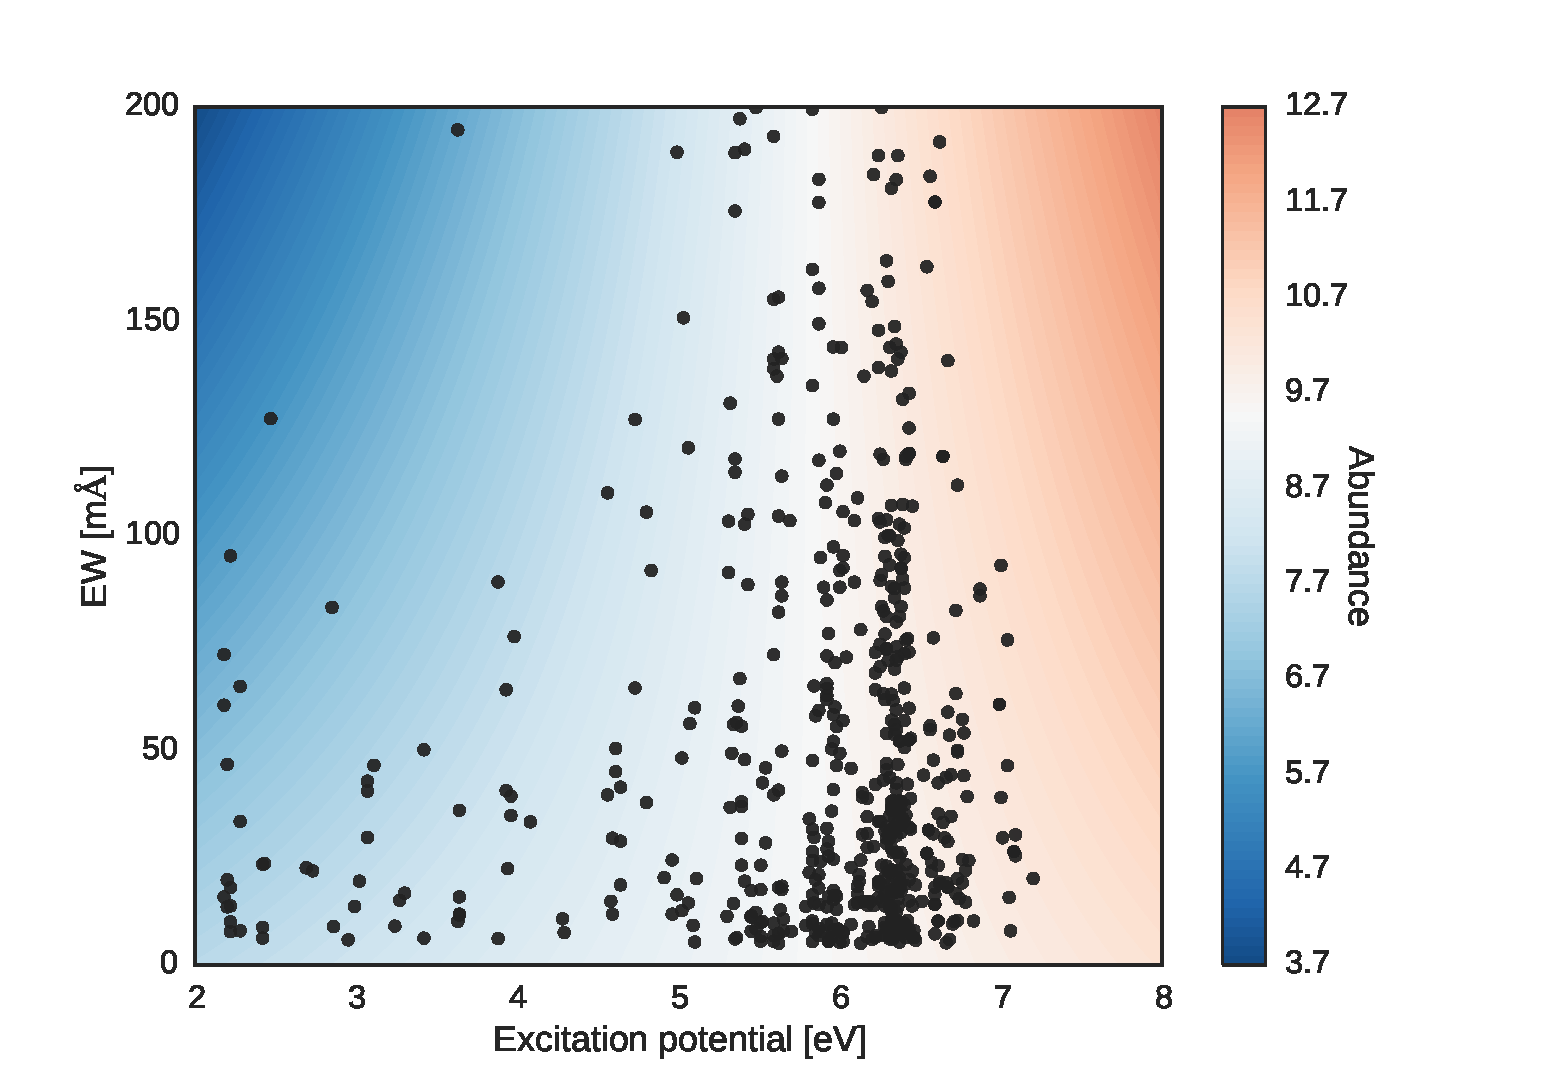
\includegraphics[width=1.0\linewidth]{figures/EWvsEP.pdf}
    \caption{The distribution of Fe I lines. At the x axis is
    the excitation potential, while the measured EWs for the Sun is
    shown at the y axis.}
    \label{fig:Fe1_before_recal}
\end{figure}


\begin{figure}[tpb]
    \centering
    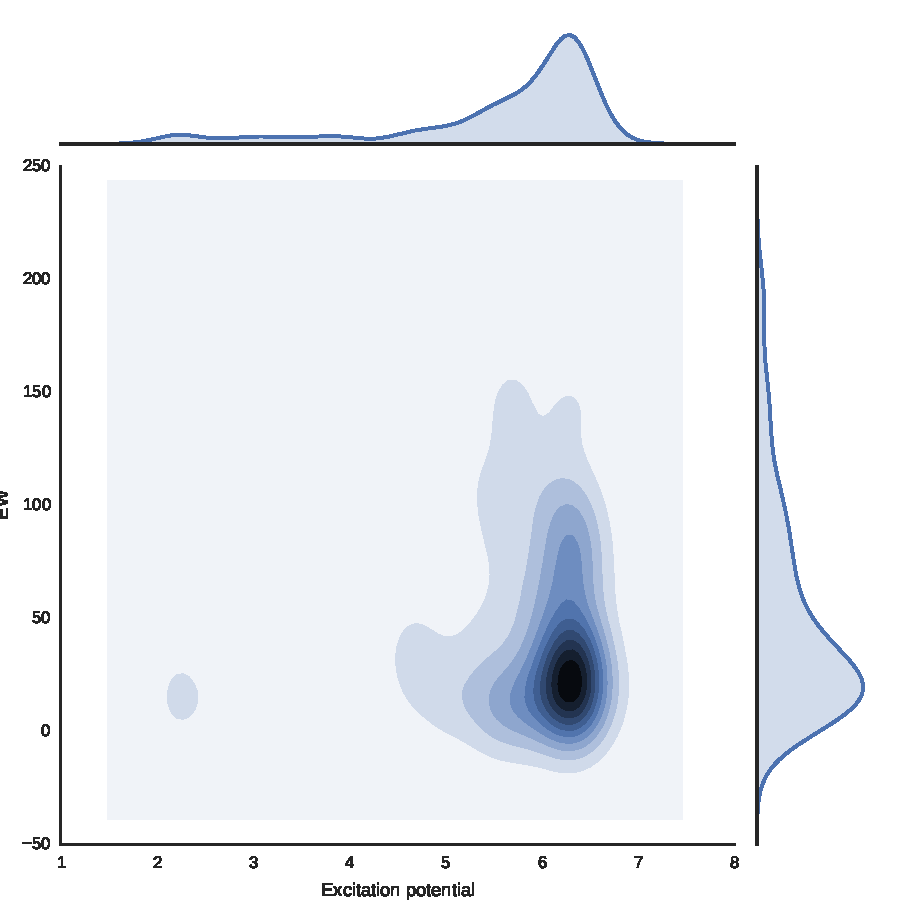
\includegraphics[width=1.05\linewidth]{figures/EWvsEP_cut.pdf}
    \caption{Distribution of both FeI and FeII lines on top of the solar
    spectrum. The distributions are after recalibration and exclusion
    of lines which deviate more than 1 dex from the expected solar iron
    abundance. There are two areas in the spectrum with high telluric
    contamination, which also mark the border between the filters we
    use: from J to H around 14000\si{\angstrom} and from H to K around
    19000 \si{\angstrom}. Most of the lines are located in the H band.}
    \label{fig:Fe1_after_recal}
\end{figure}



\subsection{Deriving parameters with the EW method}
\label{sec:deriving_parameters_with_the_ew_method}

Once the EWs have been measured for all lines in the line list (or as
many as possible), the next step is to derive atmospheric parameters.
Atmosphere models are necessary for computing abundances of the lines.
The literature offers the possibility to choose from a wide variety
of model atmospheres. Models like ATLAS9 \citep{Kurucz1993} and
MARCS \citep{Gustafson2008} are the most used atmospheric models for
derivation of spectroscopic parameters for FGK stars.

Here we use the ATLAS9 models which, for efficiency, are created
in a grid according to effective temperature, surface gravity, and
metallicity. In order to search for final parameters it is necessary to
interpolate models from the grid, thus allowing to look into a finer
grid space \citep[see e.g.][]{Sousa2014}.

For a given atmosphere model, abundances of all the lines in the line
list are calculated. By removing any correlation between the excitation
potential and abundance of all lines (from same element) the effective
temperature is constrained. In a similar way, the micro turbulence can
be constrained be removing any correlation between the reduced EW ($\log
EW$) and abundances, and the surface gravity is found when there is
ionization balance, i.e. the mean abundance of FeI and FeII are equal.
Lastly, the iron abundance comes from calculating the mean of
all the iron abundances.

When there are no longer any correlation, the final atmospheric
parameters are obtained from the atmospheric model to calculate the
given abundances.

In order to find the best atmosphere model, a minimization algorithm
is used based on the downhill simplex method \citep{Press1992} that
searches in the parameter space for the best fitting model. The
convergence criteria for the correlation between excitation potential
and abundances gives a slope less than 0.001, a slope less than 0.002
for the correlation between the reduced EW and the abundances, and a
difference of less than 0.005 between the mean abundances for FeI and
FeII.







\section{Results}
\label{sec:results}


\subsection{Derived parameters for the Sun}
\label{sec:derived_parameters_of_the_sun}

As a test, we then derived the stellar parameters for the Sun using
the resulting line-list (including the solar calibrated, astrophysical
$\log \mathrm{gf}$ values). We used the minimization procedure described
in Sect.~\ref{sec:deriving_parameters_with_the_ew_method}. Since the
line-list and $\log$ gf values has been selected using the solar
spectrum, it is with no surprise that the derived parameters for the
Sun perfectly match the adopted solar values. In addition to this, we
repeated this test but after adding noise to the EW measurements and
derived parameters with different cuts in excitation potential (EP). The
noisy EWs follow the procedure from \cite{Caryel1988}:

\begin{align}
    \sigma \simeq 1.6 \frac{\sqrt{\Delta\lambda\; \mathrm{EW}}}{\mathrm{S/N}},
\end{align}
where $\Delta\lambda=0.1\si{\angstrom}$ and we consider two different
signal-to-noise ratios, 100 and 300. This sigma is used to create a
normal distribution with a mean around the original EW.

\begin{align}
    f(x, EW, \sigma) = \frac{1}{\sqrt{2\pi\sigma^2}} e^{-\frac{(x-EW)^2}{2\sigma^2}}
\end{align}

A new set of EWs is drawn from this distribution. We make 10 different
draws for 3 different cuts in excitation potential: \SI{5.0}{eV},
\SI{5.5}{eV}, and not cut at all. This is done for both S/N considered.
This gives us 60 different line-lists, and with the original line-list
we have in total 61 line-lists. We make the cut in excitation
potential for two reasons: 1) We do not see lines with that high
excitation potential in a similar line list for the optical \citep[see
e.g.][]{Tsantaki2013} and this might be a problem for future derivation
of parameters. 2) We might have problems with the clump of lines at high
excitation potential when we try to reach iron excitation balance.

In Fig~\ref{fig:solar_parameters} the derived parameters are plotted
with different EP cuts in the line list. The horizontal black lines
are the derived atmospheric parameters without noise added to the EWs.
The color shows the two different S/N considered (blue is S/N at 100,
and green is S/N at 300). For a given S/N and EP cut, the 10 runs were
combined to a single value by calculating the mean. Additionally,
we show the 1$\sigma$ standard deviation. The derived atmospheric
parameters are presented in Table~\ref{tab:sun}.

\begin{figure}[t!]
    \centering
    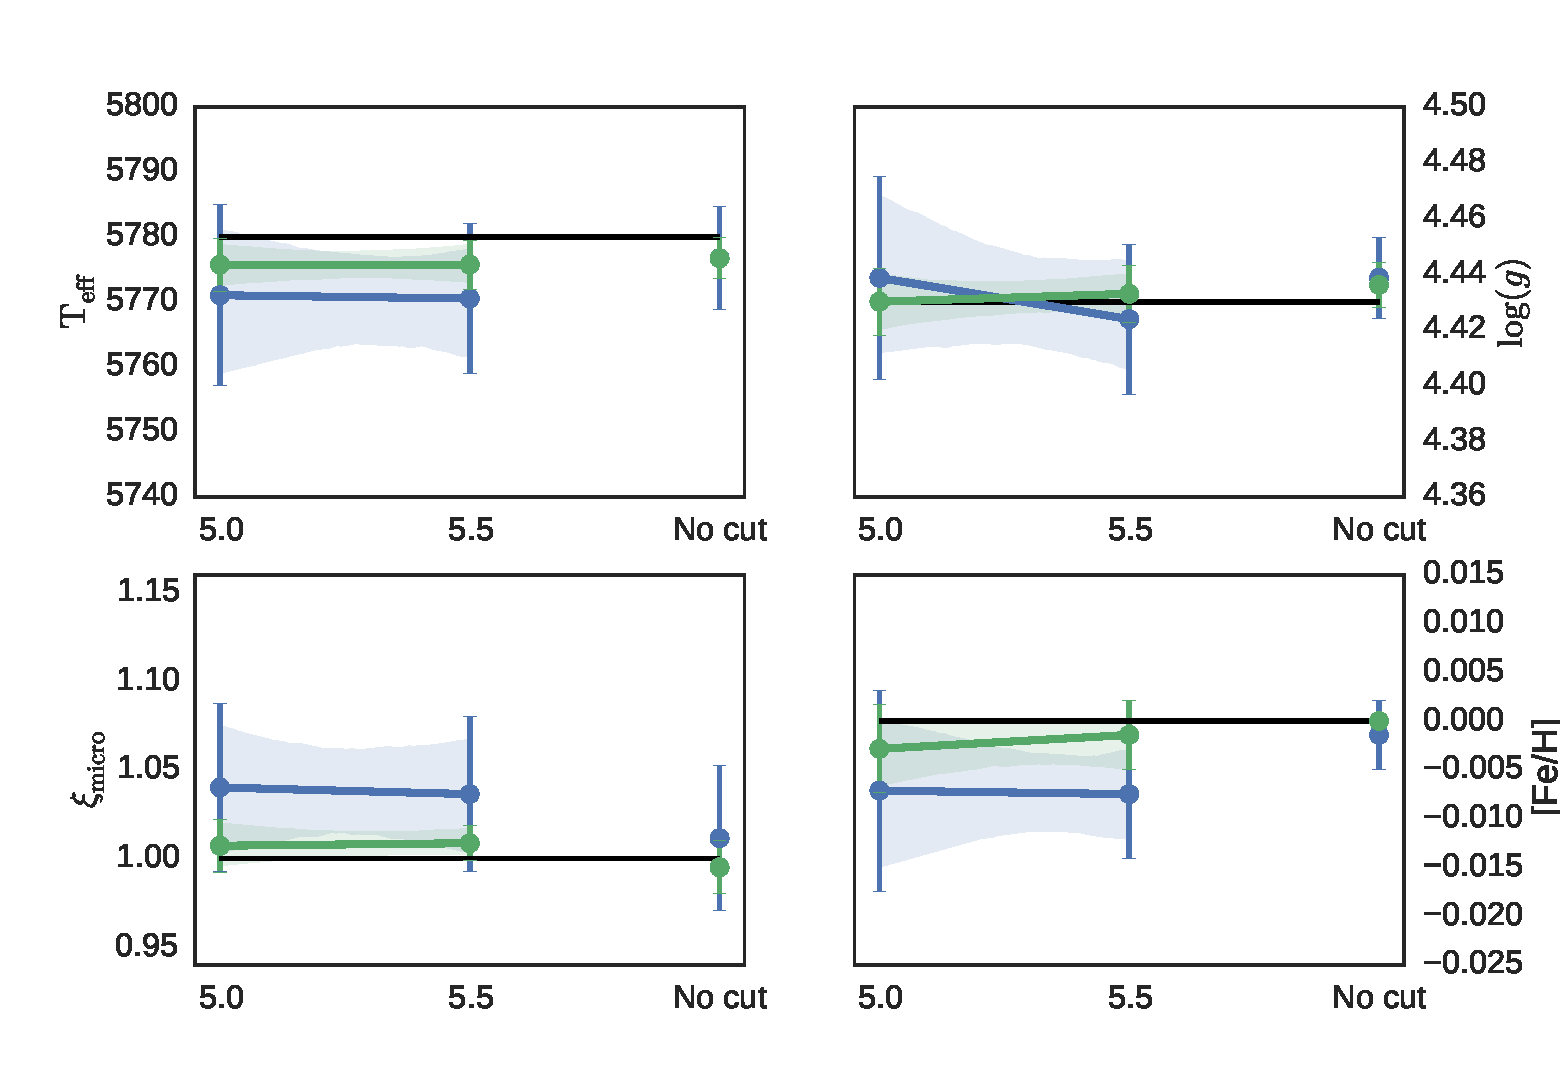
\includegraphics[width=1.0\linewidth]{figures/solar_parameters_10runs.pdf}
    \caption{Derived atmospheric parameters for the Sun. The horizontal
    black lines are the parameters for the calibrated line list, the
    three points shows the mean value of 10 runs with random noise
    added, the blue points is the results for S/N=100, while the
    green points is for S/N=300.}
    \label{fig:solar_parameters}
\end{figure}

By adding noise to the EW measurements and calculate the atmospheric
parameters with different cuts in EP, we see that the final derived parameters
are perfectly compatible with expected values.





\begin{table*}[tb!]
    \caption{The derived parameters for the Sun with two different cuts
    in EP, and with no cut. For all the line lists here, there is noise
    added to the EW measurements.}
    \label{tab:sun}
    \centering
    \begin{tabular}{llllll}
      \hline\hline
        EP cut (eV) &  S/N &  $T_\mathrm{eff}$ (K) &  $\log g$ (cgs)     &  $\xi_\mathrm{micro}$ (km/s) &  [Fe/H]           \\
        \hline
        5.0         &  100 &  $5771 \pm  41$       & $4.44   \pm  0.11$  & $1.04  \pm  0.14$            & $-0.01    \pm 0.03$\\
        5.5         &  100 &  $5770 \pm  34$       & $4.42   \pm  0.08$  & $1.04  \pm  0.13$            & $-0.01    \pm 0.02$\\
        No cut      &  100 &  $5776 \pm  23$       & $4.44   \pm  0.04$  & $1.01  \pm  0.12$            & $-0.00    \pm 0.01$\\
        \hline
        5.0         &  300 &  $5776 \pm  9 $       & $4.43   \pm  0.02$  & $1.00  \pm  0.05$            &  $0.00    \pm 0.00$\\
        5.5         &  300 &  $5774 \pm  11$       & $4.43   \pm  0.04$  & $1.01  \pm  0.04$            & $-0.00    \pm 0.01$\\
        No cut      &  300 &  $5778 \pm  9 $       & $4.44   \pm  0.01$  & $1.00  \pm  0.03$            &  $0.00    \pm 0.00$\\
      \hline
    \end{tabular}
\end{table*}




\subsection{Derived parameters for HD20010}
\label{sec:derived_parameters_of_hd20010}

At the moment of writing this paper, not many high resolution and
high signal-to-noise ratio NIR spectra are available that we can
use to test our line list. We looked into the CRIRES-POP data base
\citep{Lebzelter2012} for solar type stars. The best candidate for
testing our line list is HD20010, which resembles the Sun most in
terms of parameters. HD20010 is a well studied F8 subgiant, see e.g.
\cite{Mortier2013,Lebzelter2012}. Therefore, it is a prime object for
our studies, since we want to benchmark results from our new line list
with literature values. To analyse this star we used spectra that comes
in pieces of $\SI{50}{\angstrom}$ to $\SI{120}{\angstrom}$. The data
is not yet fully reduced. However, the data can still be used as it is
after the pipeline reduction. It is already known by the CRIRES-POP team
that the pipeline reduced form of the wavelength calibration is of poor
quality. Most of the spectra are stretched compared to e.g. a model or a
solar spectrum in the same region.

In order to measure the EWs of the lines in our line list, the
correct absorption lines need to be identified. This is done
with a software special developed for this\footnote{The software
(plot\textunderscore{}fits) is open source and can be found here:
\url{https://github.com/DanielAndreasen/astro_scripts}}. This software
does the following:
\begin{enumerate}
    \item Plot the observed spectrum.
    \item Over plot a model spectrum. In this particular the solar spectrum was
        used since the atmospheric parameters are close enough, so the sun can
        serve as a model.
    \item Over plot a telluric spectrum from the TAPAS web page \citep{Bertaux2014}.
    \item Over plot a vertical line at the location for lines in the list.
    \item Calculate the cross correlation function (CCF) for the telluric spectrum
        respect to the observed spectrum, locate the maximum value by a Gaussian fit
        and use this to shift the telluric spectrum with the found RV.
    \item Do the same as the step above, but for the model.
\end{enumerate}
The final plot shows the shifted spectra, and the CCFs at the sides. An example
of the software in use is shown in Fig.~\ref{fig:plot_fits}. The two RVs are
part of the title of the plot.



\begin{figure*}[tbp!]
    \centering
    \includegraphics[width=1.0\linewidth]{figures/plot_fits.pdf}
    \caption{The middle plot shows a piece of HD20010 (black), the model
    spectrum, in this case the Sun (green), a telluric spectrum (red), and two
    lines from our line list (magenta vertical lines). The plot to the left
    shows the CCF of the Sun with a fitted Gaussian. The right plot shows the
    same as the one to the left, but for the telluric spectrum.}
    \label{fig:plot_fits}
\end{figure*}

Once the lines are identified the EWs were measured with the splot
routine in IRAF. The reason not to choose ARES for this task was to
visually confirm the identification of the line given the relative poor
wavelength calibration at the moment. We were able to measure 249 FeI
lines and 5 FeII lines compared to 344 FeI lines and 13 FeII lines for
the Sun.

We then derived the stellar parameters using the standard procedure
(see Sect.~\ref{sec:deriving_parameters_with_the_ew_method}) as
done for the Sun. The final derived parameters for the full line
list are overestimated compared to literature values, see e.g.
\citet{Mortier2013,Gonzalez2010}. \cite{Gonzalez2010} use the same
method as us, but for an optical spectra, and derive the following
atmospheric parameters: $T_\mathrm{eff}=6170\pm33\,\si{\kelvin}$,
$\log g=3.93\pm0.02$, $\xi_\mathrm{micro}=1.70\pm0.09\,\si{km/s}$, and
[Fe/H]=$-0.206\pm0.025$. To overcome the overestimation of parameters
we tried to remove lines above different EPs and re-determine the
stellar atmospheric parameters. In this process we did not remove
any of the very few remaining FeII lines. The reason not to remove
the FeII lines is, that they are essential to determine the surface
gravity from the ionization balance. However, 5 lines were too few to
satisfactory constrain the surface gravity. To overcome this issue, we
fixed the surface gravity to the value found in \cite{Gonzalez2010}.
Fig~\ref{fig:HD20010_parameters_cuts} shows the results from this
exercise. A second degree polynomial is fitted for the effective
temperature, iron abundance, and the micro turbulence with the
95\% confidence interval. At a cut at $\SI{5.3}{eV}$ and below
the atmospheric parameters gets close to the values derived from
\cite{Gonzalez2010} which is plotted as a horizontal black line. The
exact values can be seen in Table~\ref{tab:hd20010}.


TO DANIEL:
Explain why we get so high errors. Here is a possible way to do it.

1) Take 10-15 lines with multiple EW measurements.
2) Calculate std for each line.
3) Derive parameters in the limits of the mean±std and hopefully, this can explain the high errors.

If so, the reasons for the high errors are the bad quality of the spectra at the current time.



\begin{table*}[htb!]
    \caption{The derived parameters for HD20010 at different EP cut. $\log g$
        were fixed at 3.93 for all calculations. The literature value are from \cite{Santos2004}.}
    \label{tab:hd20010}
    \centering
    \begin{tabular}{lllll}
      \hline\hline
        EP cut (eV) & $T_\mathrm{eff}$ (K) & $\xi_\mathrm{micro}$ (km/s) & [Fe/H]               \\
      \hline
        Literature  & $6170 \pm  33$       & $1.70 \pm 0.09$             & $-0.21 \pm 0.03$      \\
      \hline
        5.0         & $6112 \pm 121$       & $0.78 \pm 0.08$             & $-0.25 \pm 0.44$      \\
        5.1         & $6067 \pm 209$       & $1.39 \pm 0.17$             & $-0.29 \pm 0.74$      \\
        5.2         & $6093 \pm 196$       & $1.37 \pm 0.16$             & $-0.29 \pm 0.71$      \\
        5.3         & $6096 \pm 196$       & $1.37 \pm 0.16$             & $-0.29 \pm 0.73$      \\
        5.4         & $6294 \pm 353$       & $2.00 \pm 0.30$             & $-0.27 \pm 1.52$      \\
        5.5         & $6337 \pm 558$       & $2.14 \pm 0.49$             & $-0.26 \pm 2.48$      \\
        5.6         & $6367 \pm 714$       & $2.21 \pm 0.63$             & $-0.26 \pm 3.33$      \\
        5.7         & $6621 \pm 248$       & $2.18 \pm 0.20$             & $-0.20 \pm 1.35$      \\
        5.8         & $6624 \pm 241$       & $2.17 \pm 0.19$             & $-0.20 \pm 1.31$      \\
        5.9         & $7000 \pm 218$       & $2.09 \pm 0.09$             & $-0.11 \pm 1.29$      \\
        6.0         & $6999 \pm 181$       & $2.08 \pm 0.08$             & $-0.10 \pm 1.06$      \\
        No cut      & $7150 \pm 467$       & $2.99 \pm 0.30$             & $-0.09 \pm 3.04$      \\
      \hline
    \end{tabular}
\end{table*}



\begin{figure}[tpb!]
    \centering
    \includegraphics[width=1.0\linewidth]{figures/HD20010_parameters_cuts.pdf}
    \caption{Atmospheric parameters for HD20010. In the top panel is
    the effective temperature. The middle panel is the iron abundance,
    and the bottom panel is the micro turbulence. The parameters are
    derived with different cuts in EP. Here the horizontal black lines
    are literature values. The parameters for the full line list are
    plotted to the right for all three plots. The shaded areas are the
    95\% confidence interval for the fit.}
    \label{fig:HD20010_parameters_cuts}
\end{figure}




\section{Conclusion}
In this work, we present a new iron line list for the NIR. The quality
of the line list plays a key role for deriving atmospheric stellar
parameters. While the line list was compiled from a solar spectrum
and calibrated for the same, we tested it extensively for the slightly
hotter star, HD20010. The first results with this line list are promising.

The line list still remains to be tested for a larger sample of FGK
stars. Furthermore, it will be interesting to explore the use of this
line-list to derive parameters for M-dwarf stars using high resolution
and high S/N NIR spectra. M-dwarf stars are especially interesting
targets for an exoplanetary viewpoint, since they are prone to form low
mass exoplanets \cite{Bonfils2013}. Hence, a detailed analysis of the
host star's atmospheric parameters greatly improve our characterization
of the possible exoplanets orbiting these low mass stars. Currently,
there is one M dwarf in the CRIRES-POP, Barnard's star which will be
ideal for testing in the future.

Lastly, with the up-coming NIR spectrographs, this work and future
continuation will help the community to derive atmospheric stellar
parameters.





\begin{acknowledgements}

This work was supported by Funda\c{c}\~ao para a Ci\^encia e a
Tecnologia (FCT) through the research grant UID/FIS/04434/2013.
E.D.M, P.F., N.C.S., and S.G.S. also acknowledge the support from FCT
through Investigador FCT contracts of reference SFRH/BPD/76606/2011,
IF/01037/2013, IF/00169/2012, and IF/00028/2014, respectively, and
POPH/FSE (EC) by FEDER funding through the program “Programa
Operacional de Factores de Competitividade - COMPETE”.

This research has made use of the SIMBAD database operated at CDS,
Strasbourg (France).

\end{acknowledgements}






\bibpunct{(}{)}{;}{a}{}{,}
\bibliographystyle{aa}
\bibliography{thesis}

\end{document}
